\xchapter{Sustentabilidade do ecossistema de software acadêmico de análise estática}
{Este capítulo apresenta a avaliação do ecossistema de software acadêmico de
análise estática quanto à sua sustentabilidade técnica, ou seja, a capacidade
de perdurar, de continuar disponível no futuro, e a sua manutenabilidade.}

% Introduction
% Background
% Experimental Setup (hipoteses / design)
% Results (data analysis)
% Discussion
% Threats to validity
% Conclusions

%\section{Avaliação da sustentabilidade técnica}
%\label{sustentabilidade-tecnica}

%apesar disso, antes mesmo de resolver tais questões é
%fundamental compreender os impactos que eles causam na comunidade de pesquisa.

\section{Planejamento do estudo}

Este estudo tem como objetivo medir e avaliar a sustentabilidade técnica dos
softwares acadêmicos de análise estática publicados na literatura acadêmica.

%\subsection{Planejamento do estudo}

Coletamos para cada ferramenta selecionada suas métricas de código-fonte
através da execução da ferramenta {\it analizo metrics}, esta coleta foi
automatizada pelo script {\it
analyze-all-projects}\footnote{http://github.com/joenio/dissertacao-ufba-2016/blob/master/dataset/analyze-all-projects}
escrito durante este estudo disponível no
repositório\footnote{http://github.com/joenio/dissertacao-ufba-2016} desta
pesquisa.

\subsection{Questões de pesquisa}

Neste estudo as seguintes questões de pesquisa serão investigadas:

\begin{itemize}
  \item Os projetos tem contribuidores além dos autores iniciais?
  \item Os projetos incentivam ativamente a contribuição?
  \item Os espaços dos projetos são abertos e transparentes?
  \item Os projetos fazem um pedido explícito e claro de reconhecimento?
\end{itemize}

\newcommand{\QuestaoUm}{Na literatura científica publicada, como as taxas de
softwares publicados, no domínio de aplicação de análise estática, mudam ao
longo do tempo?}

\newcommand{\QuestaoDois}{Os softwares acadêmicos de análise estática, publicados
na literatura científica, estão disponíveis para obtenção hoje?}

\newcommand{\QuestaoTres}{Na literatura científica publicada, como as taxas de
softwares disponíveis, no domínio de aplicação de análise estática, mudam ao
longo do tempo?}

\newcommand{\QuestaoQuatro}{Podemos adaptar de forma incremental os softwares
acadêmicos de análise estática para aproveitar oportunidades emergentes, sem
perda de reprodutibilidade?}

\begin{description}
  \item [Q1:] \QuestaoUm
  \item [Q2:] \QuestaoDois
  \item [Q3:] \QuestaoTres
  \item [Q4:] \QuestaoQuatro
\end{description}

\subsection{Resultados}

\begin{enumerate}
  \item Caracterização do ecossistema de software acadêmico de análise estática
  \item Reflexão sobre os problemas de sustentabilidade sofridos pelo ecossistema de software acadêmico de análise estática
  \item Formulação de hipóteses sobre os problemas de sustentabilidade sofridos pelo ecossistema de software acadêmico de análise estática
\end{enumerate}

\section{Coleta de dados}

A população estudada compreende um conjunto de 60 projetos de software
acadêmico de análise estática publicados na literatura acadêmica de engenharia
de software.

%, dados sobre cada software acadêmico e
%informações sobre o seu ecossistema.

\subsection{Seleção de software acadêmico}

\begin{figure}[h]
  \center
  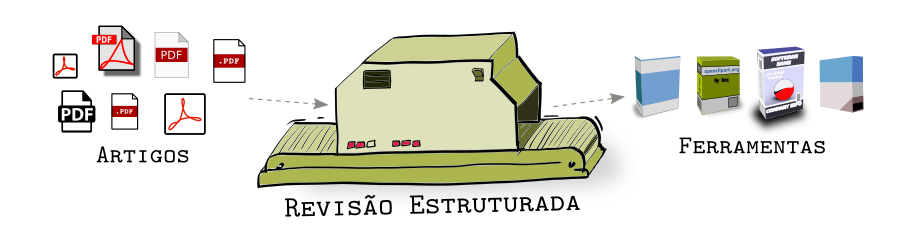
\includegraphics[scale=0.21]{imagens/revisao-estruturada.png}
  \caption{Etapas da seleção de software acadêmico}
  \label{figura-revisao-estruturada}
\end{figure}

A seleção de software acadêmico foi realizada através de um procedimento
composto de 3 etapas -- busca, filtro e seleção -- cada etapa deste
procedimento, representada na Figura \ref{figura-revisao-estruturada}, gera
como saída um conjunto de artigos utilizado como entrada na etapa seguinte, a
última etapa -- seleção -- gera como saída a nossa população de 60 projetos.

%A Tabela \ref{coding-scheme-mentions} descreve as informações
%coletadas para cada projeto.

%\begin{table}[h]
%\caption{Esquema de codificação para menções a software acadêmico como contribuição}
%\centering
%\begin{tabular}{ l p{10cm} }
%  \hline
%  Código                   & Definição \\
%  \hline
%  Nome do software         & O nome do projeto de software \\
%  URL                      & Endereço web do software ou projeto, site ou repositório de código fonte, com o software disponível \\
%  Título do artigo         & Título do artigo onde o software é citado como contribuição, seja principal ou secundária \\
%  Nome do evento           & Nome da conferência onde o software foi publicado \\
%  Ano do evento            & Ano da edição da conferência onde o artigo foi publicado \\
%  \hline
%\end{tabular}
%\label{coding-scheme-mentions}
%\end{table}

%Este esquema de codificação foi inspirado no {\it Coding scheme for mentions of
%software} proposto no trabalho de \citeonline{howison2016software}.

\subsubsection{Busca}

Nesta primeira etapa definimos as fontes utilizadas como ponto de partida para
criar o conjunto inicial de artigos onde será realizada a seleção de software
acadêmico, o principal critério utilizado na definição destas fontes é que
tenham um alto potencial de encontrar software acadêmico de análise estática
publicado como contribuição do artigo.

Este critério é avaliado de maneira subjetiva e depende do conhecimento prévio
do pesquisador e de seus pares, neste estudo selecionamos como fonte duas
conferências tradicionais da engenharia de software, SCAM - {\it Source Code
Analysis and Manipulation Working
Conference}\footnote{\url{http://www.ieee-scam.org}} e ASE - {\it Automated
Software Engineering}\footnote{\url{http://ase-conferences.org}}, ambas com um
largo histórico de publicações sobre análise de programas.

Esta primeira atividade deve incluir o maior período de tempo possível de
ediçoes de cada conferência, analisado cada edição, cada trilha, de cada uma
das conferências, ASE e SCAM, até o ano de 2015, resultando 1873 artigos em
formato PDF, cada artigo foi obtido online de forma manual através das
bibliotecas digitais disponibilizando tais publicações, cada arquivo foi
copiado localmente e organizado em diretórios separados por conferência e ano
de edição, para ser processados pela etapa seguinte. Esta etapa explorou o
histórico de 25 anos de publicação da conferência ASE e 15 anos da conferência
SCAM, representados na Figura \ref{artigos-por-ano}.

%apresenta a distribuição por edição de cada evento.

\begin{figure}[h]
  \center
  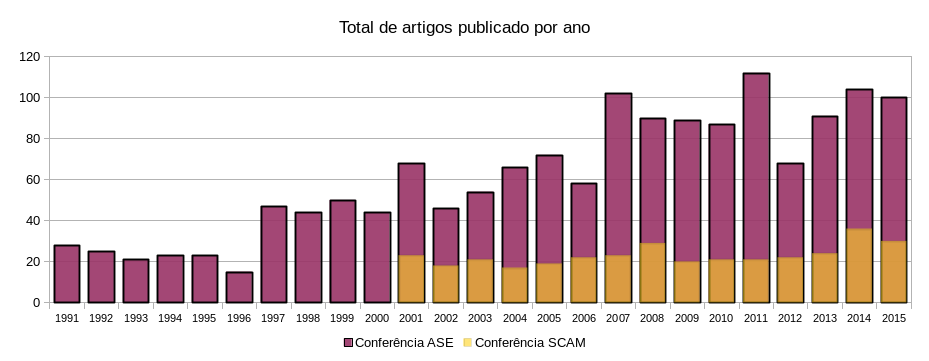
\includegraphics[scale=0.65]{imagens/artigos-por-ano.png}
  \caption{Gráfico em barras com o total de artigos publicado por ano}
  \label{artigos-por-ano}
\end{figure}

%O conjunto estudado representa um corte transversal nas publicações de dois
%eventos tradicionais da engenharia de software, análise estática, uma área com
%um bom histórico ...

\subsubsection{Filtro}

A segunda etapa reduz o número total de artigos obtidos na busca através
de um critério de corte abrangente pensado para reduzir este enorme volume
de artigos exluindo aqueles que não se enquadram nos critérios definidos
na Tabela \ref{codes-for-filter}.

\begin{table}[h]
\caption{Critérios para filtro de artigos}
\centering
\begin{tabular}{ l l l }
  \hline
  Código                          & String de filtro                   & Exemplos \\
  \hline
  Menciona software acadêmico     & {\tt tool} ou {\tt framework}         & ...      \\
  Disponibiliza online            & {\tt download} ou {\tt available}     & ...      \\
  Identifica fonte                & {\tt http} ou {\tt ftp}               & ...      \\
  Domínio de análise estática     & {\tt static analysis} ou {\tt parser} & ...      \\
  \hline
\end{tabular}
\label{codes-for-filter}
\end{table}

Estes critérios são aplicados de forma automática numa busca textual aplicada
em todo o conteúdo de cada artigo selecionado na etapa anterior, a string de
busca final tem o objetivo geral de ser abrangente a fim de evitar falsos
negativos, ou seja, evitar que o filtro deixe de fora artigos que publiquem
software de análise estática.

Esses termos devem encontrar artigos com publicação de softwares científicos do
domínio de análise estática de código fonte com disponibilidade para {\it
download}, seja binário ou código fonte, é esperado encontrar resultados com
falso positivo, ou seja, artigos com publicação de software acadêmico de outros
domínios, ou artigos com publicação de software acadêmico mas sem menção
à fonte online para obtenção, entre outras situações.

Nesta reduzimos o conjunto total de artigos para 441 artigos, a etapa seguinte
identificará os possíveis falsos negativos deste conjunto reduzido deixando-os
fora do resultado final.

\subsubsection{Seleção}

Na terceira e última etapa avaliamos se, de fato, os artigos contribuem com software
acadêmico de análise estática dentro dos critérios de disponibilidade
descritos na Tabela \ref{codes-for-selecao}.

\begin{table}[h]
\caption{Codes for functions \cite{howison2016software}}
\centering
\begin{tabular}{ l p{12cm} }
  \hline
  Código           & Explicação \\
  \hline
  Identificável    & É possível identificar o nome do software acadêmico (ex, Existe um nome, ... "um programa que nós escrevemos?" Podemos encontrar referencias para o software, mesmo que o software não seja encontrado?) \\
  Encontrável      & Uma vez que o software é identificável, podemos encontrar uma fonte online que detalha o software (não necessariamente o próprio software, mas alguma presença oficial) (ex, a página do projeto ou manual online)? \\
  Disponível       & Os autores informam uma URL para obtenção online do software acadêmico \\
%  \item Os autores descrevem o software acadêmico como uma das contribuições do estudo
  \hline
\end{tabular}
\label{codes-for-selecao}
\end{table}

Esta seleção é feita a partir de uma leitura superficial do artigo incluindo
título, introdução, resultados e conclusões, o objetivo é identificar se o
artigo publica software acadêmico e indica onde obter uma cópia do software.

Quando esta leitura inicial não é o suficiente para
identificar se há publicação de software, outras seções são lidas, alguns
artigos descrevem a implementação do software em seções específicas, outros
indicam detalhes do software ao longo do texto, é comum o uso de
notas de rodapé para indicar onde o software está disponível. Software
acadêmico que seja mais abrangente do que apenas análise estática de
código fonte mas que contenham esta função em seu conjunto também são
selecionados.

\begin{figure}[h]
  \center
  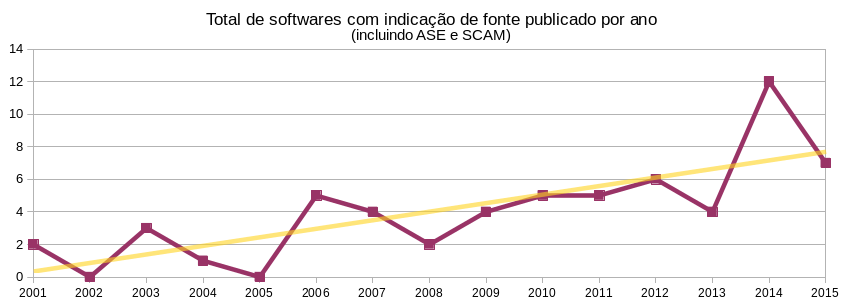
\includegraphics[scale=0.65]{imagens/softwares-por-ano.png}
  \caption{Gráfico em linha com o número total de resultados por ano}
  \label{softwares-por-ano}
\end{figure}

Nesta última etapa selecionamos 62 artigos mencionando como uma das
contribuições um software acadêmico, identificado com nome e URL, disponível
para download segundo seus autores. Dois dos resultados de software acadêmico
encontrados são mencionados em dois artigos, resultado ao final 60 projetos de
software acadêmico, apresentados na Figura \ref{softwares-por-ano}
distribuídos por ano.

\subsection{Caracterização dos projetos selecionados}

Cada software acadêmico selecionado foi caracterizado com informações obtidas a
em fontes documentais diversas, como, artigos onde o software foi selecionado,
fonte online sobre o projeto, site ou repositório de código fonte, manuais, e o
próprio código fonte quando disponível, as informações coletadas, descritas na
Tabela \ref{coding-scheme-software}.

\begin{table}[h]
\caption{Esquema de características coletadas para cada software acadêmico}
\centering
\begin{tabular}{ l p{11cm} }
  \hline
  Código                   & Explicação \\
  \hline
  Nome do software         & O nome do projeto de software \\
  Descrição do software    & A descrição do projeto de software \\
  URL                      & Endereço web do software ou projeto, site ou repositório de código fonte, com o software disponível \\
  Título do artigo         & Título do artigo onde o software é citado como contribuição, seja principal ou secundária \\
  Nome do evento           & Nome da conferência onde o software foi publicado \\
  Ano do evento            & Ano da edição da conferência onde o artigo foi publicado \\
  Código fonte disponível  & É possível acessar o código fonte de alguma forma? \\
  Acesso                   & Podemos acessar o software agora? Pode receber os seguintes valores: Sem Acesso, Acesso Pago, Acesso Gratuito \\
  Distribuição             & Como o software é distribuído e pode ser acessado? Pode receber os seguintes valores: gratis, foss, proprietário \\
  Licença                  & O software deixa explícito qual licença é distribuído? \\
%  Permissão para modificar & Os criadores dão permissão para modificar o programa (se não menciona modificação, assume não)?; se permissão apenas por contato, também não \\
  Código fonte             & Em qual linguagem de programação o software acadêmico foi desenvolvido \\
  Entradas suportadas      & Qual o tipo de entrada suportada pelo software de análise estática \\
  Linguagens suportadas    & Quais linguagens de programação o software de análise estática suporta como entrada \\
  \hline
\end{tabular}
\label{coding-scheme-software}
\end{table}

Os softwares disponíveis foram avaliados em relação à disponibilidade de código
fonte e à licença utilizada, essas informações, ...

A ferramenta livre {\it sloccount}\footnote{http://www.dwheeler.com/sloccount}
foi utilizada para identificar a linguagem de programação em que cada software
é escrito.

\subsection{Citações e menções}

Coletamos também para cada software acadêmico todas as menções encontradas nas
bibliotecas digitais IEEE Explore e ACM, a busca foi realizada usando o nome do
software, uma string de busca foi criada usando o nome do software e quando
necessário compondo com outras características, alguns exemplos de strings de
busca são apresentados na Tabela \ref{exemplos-strings}.

\begin{table}[h]
\caption{Exemplos de strings de busca por menções}
\centering
\begin{tabular}{ l p{10cm} }
  \hline
  Software acadêmico & String de busca no IEEE Xplore e ACM \\
  \hline
  CodeBoost          & {\tt ((CodeBoost) AND C++)} \\
                     & {\tt content.ftsec:(+CodeBoost +"C++" +Tool)} \\
  \hline
  TestEra            & {\tt (((((TestEra) AND framework) AND Java) AND testing) AND sarfraz)} \\
                     & {\tt content.ftsec:(+TestEra +framework +Java +testing +sarfraz)} \\
  \hline
  XOgastan           & {\tt (XOgastan)} \\
                     & {\tt content.ftsec:(+XOgastan)} \\
  \hline
\end{tabular}
\label{exemplos-strings}
\end{table}

Todos os resultados, do IEEE e ACM, foram agrupados num único arquivo no
formato BibTeX, as duas bibliotecas possuem a opção de fazer download do
resultado de uma busca neste formato de arquivo, os resultados foram unificados
para reduzir duplicidades.

Para cada resultado copiamos localmente o artigo em formato pdf, cada artigo
foi lido em busca de encontrar menções ao nome do software,
em qual contexto o software é mencionado e de que forma é mencionado,
a Tabela \ref{coding-scheme-mention} resume cada
tipo de menção com explicação dos casos em que se enquadram,
o método utilizado
para esta busca foi realizado com auxílio do mecanismo de busca do leitor de
pdf\footnote{Utilizamos o software livre Evince versão 3.22.1} utilizado para
leitura dos artigos, com o auxílio da busca encontramos cada ocorrência ao nome
do software tomando nota sobre o contexto e o uso que é feito do software neste
contexto.

\begin{table}[h]
\caption{Tipos de menções ao software acadêmico encontrados nos artigos}
\centering
\begin{tabular}{ l c p{10cm} }
  \hline
  Tipo da menção   & Peso & Explicação \\
  \hline
% * tipo e peso da citação (peso em ordem crescente)
  Cita o software  & 0.1    & Apenas cita o software ou é o mesmo artigo onde o software selecionado; É um artigo com ``mesmo'' conteúdo publicado na ``mesma'' época; O artigo apenas descreve o software; Menciona o software numa tabela com outros, classifica; Menciona o software como exemplo; Menciona o software como trabalho relacionado; Menciona o software em trabalhos futuros \\
  Usa o software   & 0.25    & Avalia ou caracteriza o software; Usa para coleta ou análise de dados; Usa como objeto de estudo; Usa o software como parte de uma solução, implementação, etc; Cria um software derivado mas não disponibiliza as contribuições \\
  Contribui ou integra & 0.5 & Contribuição pequena ou moderada; Extende o software; Integra o software a outros sistemas, formatos de entrada/saída, APIs, etc (seja implementando suporte no software ou do outro lado); Refatora parte do software; Implementa parte do software em outro projeto e compara resultados \\
  Contribui ou cria & 1 & Cria; Contribuição inicial criando o projeto; Faz uma grande contribuição; Refatora todo o software; Abre o código de um software que antes era de código fechado \\
  \hline
\end{tabular}
\label{coding-scheme-mention}
\end{table}

Como os resultados da busca foram copiados em seu formato BibTeX diretamente
das bibliotecas digitais, temos para cada um dos artigos todos os seus
metadados, autores, ano de publicação, conferência, jornal, etc. Os autores de
cada uma das menções ao software, por exemplo, serão utilizados na fase de
análise para calcular o quanto de autores novos começaram a publicar sobre
certo software acadêmico.

\subsection{Métricas de software}

Coletamos métricas de produto e projeto de cada software, como, número total de
lançamentos, datas e versões de cada lançamento, número de commits no
repositório git e calculamos a complexidade estrutural do código fonte do
software.

As informações de lançamentos, versões e datas de cada lançamento foram coletadas
manualmente, geralmente disponíveis em arquivos de changelog ou em tags no
repositório de código fonte.

O número de commits foi agrupado por ano, para cada software, apenas entre os
que estão disponível em repositórios git, coletamos o número total de commits
realizado e agrupamos por ano.

Os softwares com código fonte disponível foi coletado a métrica de complexidade
estrutural. A coleta dessa métrica foi realizada pelo Analizo, uma suíte de
ferramentas para análise de código fonte, apresentada em detalhes no Capítulo
\ref{analizo}.






%\section{Análise dos dados}
\section{Resultados}

os nomes dos autores foram normalizados,
e para cada artigo citando um software extraimos e identificamos o nível
de ineditismo daqueles pesquisadores com aquele software, os valores
são os seguites:

e as demais coletadas até aqui,
foram distribuídas cronologicamente, e interpretadas numa perspectiva histórica
sobre a sustentabilidade técnica dos softwares acadêmicos de análise estática.

\begin{table}[h]
\caption{Autoria das menções ao software acadêmico encontradas nos artigos}
\centering
\begin{tabular}{ l c p{10cm} }
  \hline
  Novos atores no ecossistema & Peso & Explicação \\
  \hline
  Criadores & 0 & São os primeiros autores a publicar sobre o software \\
  Nenhum    & 0.1 & Todos os autores já publicaram sobre o software em anos anteriores \\
  Parte     & 0.25 & Uma parte dos autores já publicou sobre o software em anos anteriores \\
  Todos     & 0.5 & Nenhum dos autores jamais publicou sobre o software \\
  \hline
\end{tabular}
\label{coding-scheme-author}
\end{table}

Escala de peso da autoria ... Tabela \ref{coding-scheme-author} ...

%\subsection{Seleção de software acadêmico}

%A revisão estruturada difere da revisão e do mapeamento sistemático
%\cite{Kitchenham2007} por ser um processo mais simples e menos rígido, onde o
%resultado final é um conjunto de softwares, enquanto no mapeamento ou na
%revisão sistemática há um esforço em caracterizar os artigos analisados o mesmo
%não ocorre na revisão estruturada, onde o esforço reside em caracterizar os
%softwares acadêmicos.

Ao final da revisão poderemos responder à questão de pesquisa {\bf Q1}
(\QuestaoUm) usando os dados dos softwares acadêmicos selecionados.

%\subsection{Quantificação da disponibilidade dos softwares acadêmicos}

Isto nos permitirá responder as questões de pesquisa {\bf Q2} (\QuestaoDois)
e {\bf Q3} (\QuestaoTres).

%Mesmo que o autor tenha disponibilizado fontes para obtenção dos artefatos produzidos,
%o fato de não informarem a fonte inviabiliza, ou ao menos dificulta, bastante
%pesquisadores interessados em repetir ou reproduzir os resultados de tais estudos.

A avaliação sobre a disponibilidade de código fonte nos permitirá responder a questão de pesquisa
{\bf Q4} (\QuestaoQuatro).

secao: identificando menção aos softwares acadêmicos selecionados

4º Princípio, Persistencia

Os identificadores únicos e metadados descrevendo o software e sua disposição
devem persistir - mesmo além do tempo do software que descrevem.

Acesso ao software

5º Princípio da citação à softwares, Acessibilidade:

``citações aos softwares devem permitir e facilitar acesso ao software,
metadados, documentação, dados e outros materiais necessários tanto
para humanos quanto para máquinas se informar do referido software''

Não significa que o software deva estar disponível gratuitamente, mas que
os metadados devem prover informação suficiente para que o software seja
acessado. Se o software é livre, os metadados devem prover um identificador
que pode ser resolvido para uma URL apontando para a versão específica
do software sendo citado.

Pra softwares comerciais, os metadados devem ainda prover informações sobre
como acessa o software, mas pode ser um número de telefone da empresa que
vende o software ou o link para um site que venda o software

\cite{smith2016software}

5. Accessibility: Software citations should facilitate access to the software itself and to its


cada citação pontua no máximo 1 ponto para o peso final do paper ao quanto
contribui para a sustentabilidade técnica do software, esta pontuação será
calculada com base nos pesos (em porcentagem) 'contribution\_weight' e
'authorship\_weight', este último valor é aplicado à contribution weight,
ou seja contribution\_weight é acrescido a partir do valor de authorship\_weight.
o valor final se ultrapassar 1 será cortado no limite 1 (máximo), a ideia não é muito
os números, não queremos saber se são numeros altos, queremos constancia, queremos
medir se existe um nível de contribuição mínimo aos softwares, isto está
sendo proposto como algo que mantém o software vivo e útil para a comunidade
acadêmmica. (por hora o valor mínimo "ideal" por ano é "0.5", ou seja, um
valor bem modesto, este valor indica que houve ao menos uma contribuição
ao software, ou que teve citações suficientes equivalente a uma contribuição,
o software ao ser muito citado ganha mais visibilidade, impacta na possibilidade
de maior adoção e maior contribuição por terceiros.

outro fator de peso para definir o valor final do peso é se houve lençamentos
de novas versões do software naquele ano, se houve ao menos 1 versão lançada,
isso leva o final\_weight para o valor máximo 1.0 (que representa 100\%)



%\subsection{Quantificação da disponibilidade dos softwares acadêmicos}

%\section{Resultados}

Todas as trilhas de ambas as conferências
foram incluídas, encontramos nesta atividade 1873 artigos no total, 1527 artigos
do ASE e 346 artigos do SCAM, com uma média geral de 75 artigos publicados por ano. A
Figura \ref{artigos-por-ano} apresenta a distribuição por edição de cada
evento.

(1) Busca -- Todas as trilhas de ambas as conferências foram incluídas,
encontramos nesta atividade 1873 artigos no total, 1527 artigos do ASE e 346
artigos do SCAM, com uma média geral de 75 artigos publicados por ano. 

Entre os anos de 1991 e 1996 a conferencia ASE chamava-se KBSE - {\it
Knowledge-Based Software Engineering Conference} e só a partir de 1997 passou a
chamar-se ASE - {\it Automated Software Conference}. A edição com o maior
número de publicações foi 2011 com 112 artigos publicados, seguido de 2014 com
104, e 2007 com 102, a edição com o menor número foi 1996 com apenas 15 artigos
publicados.

A conferência SCAM teve sua primeira edição apenas em 2001, 10 anos após a
primeira edição do ASE, e possui uma média de 23 artigos publicados por edição.
Se compararmos os mesmos períodos de ambas as conferências, 2001 à 2015,
percebemos que a conferência ASE publica quase 4 vezes mais do que a
conferência SCAM. Neste período a conferência ASE teve uma média de 80 artigos
publicados por ano, se for levado em conta todas as edições, apenas da
conferência ASE, a média cai para 61 artigos por ano.

(2) Filtro -- reduziu em 77\%
o número total de artigos, resultando em ??? (metodologia) artigos
para serem analisados na próxima etapa da revisão estruturada.  Durante a execução desta
atividade foi necessário analisar dois artigos manualmente, {\it Adaptable
concern-based framework specialization in UML} e {\it Property-oriented test
generation from UML Statecharts}. O conteúdo destes dois artigos não é possível
de ser analisados pelo script de filtro uma vez que é formado por imagens
digitalizadas, ambos artigos publicados no ASE edição 2004. Nenhum dos dois
artigos continham os termos pesquisados e ficaram fora do conjunto selecionado
nesta atividade.

A terceira e última atividade da revisão estruturada -- (3) Seleção --
realizada em cima dos 441 artigos selecionou 107 artigos com publicação de
software científico do domínio de aplicação de análise estática, alguns destes
artigos fazem referência à um mesmo software, é o caso do {\it BEST: A symbolic
testing tool for predicting multi-threaded program failures} e do {\it Scalable
and precise symbolic analysis for atomicity violations}, ambos publicados no
ASE 2011 fazem referência ao software BEST. Situação similar ocorreu com o {\it Augmenting
Counterexample-Guided Abstraction Refinement with Proof Templates} e o {\it
PtYasm: Software Model Checking with Proof Templates} publicados no ASE 2008,
fazem referência ao software PtYasm. Por conta disso, entre os 107 artigos, temos
105 softwares distintos, uma lista com todos os softwares e uma breve descrição
de cada um é apresentado no Apêndice \ref{resumo-softwares},
detalhes sobre o número de artigos e softwares encontrados em cada conferência
pode ser consultados nos Apêndices \ref{artigos-do-scam} e \ref{artigos-do-ase} 

Ainda durante esta última atividade da revisão cada um dos 107 artigos foram
analisados em busca de informações sobre onde encontrar o software indicado,
esta análise resultou em 60 softwares com indicação de fonte para obtenção do
software, apenas os artigos que indicam endereço de página web para download do
software foram selecionados, ou seja, uma grande parte dos artigos que produzem
softwares acadêmicos nem ao menos citam o software no paper, ou quando citam,
não informam site ou endereço do projeto para download
\cite{allen2017engineering}, seja código fonte ou apenas binários.

É possível perceber um certo crescimento no número de softwares publicados com
o passar dos anos, ao menos em softwares do domínio de análise estática, de
forma que podemos confirmar que considerando as conferências ASE e SCAM, há um
crescimento na publicação de softwares acadêmicos ao longo do tempo, nos dando
oportunidade de responder parte da questão de pesquisa {\bf Q1} (\QuestaoUm).

Apesar da busca na atividade -- (2) Filtro -- utilizar termos com o objetivo de
encontrar apenas softwares disponíveis com informação de onde encontrar o
software, ainda assim, encontramos 45 artigos com publicação de software sem
indicação de fonte para obtenção.

Entre os 1873 artigos, encontramos 107 artigos referenciando 105 softwares de
análise estática, apenas 60 destes indicam fonte onde o software pode ser
encontrado, apenas 37 estão disponíveis, os 23 restantes indicam fonte não mais
acessíveis, endereço não encontrado, indisponível, ou com informações não
relacionadas ao software. O Apêndice \ref{resumo-softwares-disponiveis} traz
uma tabela com os nomes e endereços web onde os softwares estão disponíveis.

Esta informação nos permite responder a questão de pesquisa {\bf Q2}
(\QuestaoDois), levando em conta a sustentabilidade técnica podemos responder que 61\% dos
softwares produzidos no domínio de aplicação de análise estática são
sustentáveis, ou seja, continuam disponíveis ao longo do tempo. Lembrando que
não está sendo considerado aqui pesquisas que publicam software sem menção à
fonte onde pode ser encontrado o software, a revisão estruturada teve como foco encontrar
artigos com publicação softwares com indicação de fonte, ou seja, aqueles
artigos que publicam software mas que não indicam fonte não está sendo
considerado aqui, vimos que na revisão estruturada, mesmo não sendo o objetivo
encontramos 45 artigos sem informação de fonte, isto faria esta taxa cair para
apenas 35\%, uma revisão estruturada mais abrangente com objetivo de encontrar
todo e qualquer software, independente de indicar fonte ou não, com certeza
faria esta taxa cair abaixo dos 35\%, indicando que o número de softwares
publicados e hoje indisponíveis é maior que os números encontrados neste estudo.

\citeonline{robles2010replicating} afirma que existe uma tendência das páginas
web onde os softwares estão disponíveis tem uma grande chance de se tornarem
indisponíveis ao passar do tempo, podemos investigar esta tendência 
avaliando os 60 softwares com fonte indicada no artigo,
identificar se confirmamos neste contexto se com a idade do paper
as páginas web onde os softwares são publicados tem uma grande chance de se
tornarem indisponíveis ao passar do tempo.

\begin{figure}[h]
  \center
  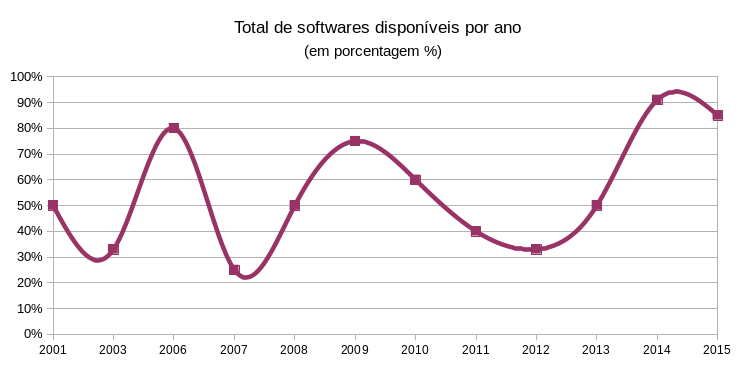
\includegraphics[scale=0.65]{imagens/softwares-disponivel-por-ano.png}
  \caption{Gráfico em linha com o total de softwares disponíveis por ano}
  \label{softwares-disponivel-por-ano}
\end{figure}

A Figura \ref{softwares-disponivel-por-ano} apresenta em cada ano quantos
porcentos do total de softwares publicados com indicação de fonte estão ainda continuam
disponíveis hoje, ou seja, quantos qual é a taxa de softwares que continuam
disponíveis hoje dentro do conjunto de softwares publicados em cada ano com
informação sobre fonte para download.  Os anos de 2002, 2004, 2005, e
anteriores a 2001 não possuem softwares publicados com fonte indicada no artigo
ainda disponível, portanto não constam no gráfico suas informações.

Ao analisar a figura percebemos que há um leve crescimento na disponibilidade
dos softwares nos anos mais recentes, com isso podemos responder à nossa
questão de pesquisa {\bf Q3} (\QuestaoTres).

Existe uma leve tendência da fontes informadas, páginas web, se tornarem
indisponível ao longo do tempo, é possível notar que em 2006 80\% de todos os
softwares de análise estática publicados estão ainda disponíveis, este número
cresce em 2014 chegando a 90\%, e cai no ano seguinte para 85\%, apesar de não
estar sempre crescente, e de termos uma amostra pequena, apenas 60 softwares,
este leve indício confirma a afirmação de \citeonline{robles2010replicating}.

Esses 37 softwares com fonte disponível foram avaliados em relação ao segundo
aspecto em respeito à de que forma estão disponíveis, os artigos informam onde
obter tais softwares, os softwares estão realmente disponíveis, as fontes
indicadas foram acessadas e na presente data deste trabalho estão funcionando e
acessíveis


Entre estes apenas 3 não possuem código fonte disponível, 34 estão com o código
fonte disponível publicamente, dentre elas 13 não informam licença alguma
apensar de ter o código fonte disponível, 21 informam licenças de FOSS ({\it
free and open source software}):

\begin{itemize}
  \item 8 usam GNU General Public License;
  \item 2 usam Apache License;
  \item 4 usam BSD License;
  \item 3 usam Eclipse Public License;
  \item 2 usam University of Illinois/NCSA Open Source License;
  \item 1 usa licença {\it FrontEndART Software Ltd}; e
  \item 1 usa licença {\it SAnToS Laboratory Open Academic License}.
\end{itemize}

Com essas informações podemos responder à terceira e última questão de
pesquisa desse estudo {\bf Q4} (\QuestaoQuatro).

Entre os 37 softwares disponíveis 21 podem ser modificados para se adaptar às
necessidades emergentes sem necessidades de solicitação prévia de autorização
aos autores originais devido ao uso de licenças livres. Os 13 softwares
restantes com código fonte disponível mas sem licença expressa podem
eventualmente serem modificados mas a falta de uma licença impõe à necessidade
de solicitar permissão aos autores originais.

35\% dos softwares disponíveis podem ser adaptados de forma incremental para
aproveitar oportunidades emergentes, 21\% podem mediante prévia autorização do
autor original serem modificados, e apenas 5\% não oferecem essa possibilidade
por não disponibilizarem o código fonte publicamente.

\section{Ameaças à validade}

Estamos considerando que o código fonte é necessário para repetir um dado
estudo mas pode ser que em alguns casos o estudo possa ser repetido mesmo sem a
disponibilidade do mesmo, isto poderia ser resolvido realizando a repetição
de cada estudo na prática e a partir daí identificar se o código fonte dos
softwares desenvolvidos são requeridos.

A escolha de um domínio de aplicação específico para seleção dos softwares
pode ser um fator de influencia nos resultados obtidos, sendo possível que
o número de artigos com publicação de softwares com código fonte disponível
encontrado não reflita nos outros domínios, os problemas diagnosticados
neste domínio pode não ser verdade em outros domínios, sendo necessário
realizar o mesmo estudo em outros domínios.

A leitura dos artigos na revisão estruturada para identificar se publicam
softwares de análise estática de código fonte, se disponibilizam fonte para
obtenção de tais softwares, e se os softwares são mesmo do domínio de aplicação
de análise estática de código fonte podem ter maior validade se feitos em
par e revisados por outros pesquisadores, neste estudo tudo foi feito pelo
autor deste estudo e não houve revisão por pesquisadores independentes.

\section{Conclusões}

Dos 346 artigos do SCAM e 1533 artigos do ASE analisados na revisão estruturada
apenas 44\% (155 artigos) e 18\% (281 artigos) continham os termos pesquisados
no filtro automático da segunda atividade da revisão, respectivamente.

Deste total apenas 11\% (41 artigos) e 4\% (62 artigos) foram selecionados na
terceira e última atividade da revisão contendo publicação de ferramenta de
análise estática.

Resultando em 103 artigos com publicação de {\it software científico} de
análise estática de código fonte, apenas 35 possuem fonte para obtenção do
software, sendo 32 de código aberto, ou seja, com disponibilidade de
código fonte, e 3 grátis, apenas binários disponível. Ou seja, apenas 31\% dos
artigos com publicação de software disponibilizam o código fonte das mesmas.
Isto significa que 69\% dos artigos com publicação de software de análise
estática de código fonte são potencialmente impossíveis de serem repetidos, já
que os artefatos originais são necessários para tal atividade e o artigo não
disponibiliza o código fonte dos mesmos.

% o artigo com resumo do RESER 2011 diz \cite{knutson2010report}:
% 4) Re-
% search tools are either not available or not usable, so precise
% replication is impractical [1, 2, 8, 18, 19].

Muitos outros aspectos podem ser levados em consideração quando se está
avaliando a capacidade de repetir ou replicar um estudo, aqui avaliamos apenas
a disponibilidade de código fonte dos softwares científicos, mas inúmeros detalhes
pormenores são necessários, tais como: indicar qual versão do software foi
utilizado no estudo, 

No entando, consideramos que nem todos os scripts e código fonte pode
valer o custo de dua publicação, sabe-se que umas das barreiras para publicação
de muitos destes artefatos são as dificldades em tal atividade,
e as objeções a tal prática de ter RR reques um esforço adicional \cite{madeyski2017would},
em muitos
estudos o simples fato de não possuir código disponível pode não levar
a problemas para alcançar a meta final que é aumento da validade do estudo,


Todas as atividades e artefatos produzidos neste estudo estão documentados em
repositório público no
Github\footnote{\url{http://github.com/joenio/dissertacao-ufba-2016}}, o
Apêndice \ref{apendice-revisao-estruturada} traz mais informações.

%, uma lista completa e
%o endereço de cada edição onde os artigos foram obtidos está documentado no
%Apêndice \ref{edicoes-conferencias}

%% usar a dimensao abaixo para definir quais usar na avaliacao longitudinal:
%% 
%% %, e qual a frequência de lançamentos indicando se são
%% %atualizadas frequentemente ou estão obsoletas.
%% 
%% \begin{description}
%% 
%%   \item {\it Lançamentos ({\it Releases}) - quantos lançamentos por ano:}
%%     \begin{itemize}
%%       \item Frequentemente $>=$ 3 vezes ao ano\\
%%         {\it \small novas versões da ferramenta são lançadas 3 ou mais vezes por ano}
%%       \item Ocasionalmente $<$ 3 vezes ao ano\\
%%         {\it \small novas versões da ferramenta são lançadas menos que 3 vezes ao ano}
%%       \item Obsoleta 0 vezes ao ano\\
%%         {\it \small intervalo entre novos lançamentos é maior que 1 ano}
%%     \end{itemize}
%% 
%% \end{description}
%% 
%% O autor não deixa claro como categorizar softwares sem lançamentos nos últimos
%% anos mas com histórico de lançamento frequente em anos anteriores. Assim, será
%% considerado todo o histórico de lançamentos e só serão considerados obsoletos
%% por exemplo softwares que nunca tenha tido mais de 1 lançamento ao ano
%% considerando todo o histórico dele. Da mesma forma, será considerado ocasional
%% apenas aqueles que sempre tiveram no máximo 2 lançamentos ao ano. Esta dimensão
%% irá nos dizer o grau de evolução de cada ferramenta, considerando que softwares
%% com lançamentos frequentes estão evoluindo.
%% 
%% ======================
%% 
%% \begin{description}
%% 
%%   \item {\it Entrada - quais tipos de arquivos podem ser carregados na ferramenta:}
%%     \begin{itemize}
%%       \item Código-fonte - arquivos de código texto podem ser carregados
%%       \item Byte code - arquivos com Java Byte Code ou Microsoft
%%       \item Linguagem intermediária (MSIL) pode ser carregada
%%     \end{itemize}
%% 
%%   \item {\it Linguagens suportadas - quais linguagens de programação a ferramenta suporta:}
%%     \begin{itemize}
%%       \item .NET - todas as linguagens compiladas em bibliotecas ou programas no framework .NET
%%       \item VB .NET - suporta VB.NET
%%       \item C\# - suporta C\#
%%       \item Java - suporta linguagem de programação Java
%%       \item C, C++ - suporta linguagem de programação C ou C++
%%     \end{itemize}
%% 
%% \end{description}
%% 
%% As dimensões apresentada por \citeonline{Novak2010} não cobrem alguns aspectos
%% importantes percebidos ao longo deste estudo, assim novas dimensões serão utilizadas
%% em complemento às dimensões citadas acima.
%% 
%% \begin{description}
%% 
%%   \item {\it Linguagem de programação - em que linguagem de programação à ferramenta é escrita:}
%%     \begin{itemize}
%%       \item .NET
%%       \item VB .NET
%%       \item C\#
%%       \item Java
%%       \item C, C++
%%     \end{itemize}
%% 
%% \end{description}
%% 
%% =============
%% 
%% \subsection{Ferramentas da indústria}
%% 
%% Em paralelo à revisão estruturada para seleção de ferramentas da academia
%% foi realizada uma seleção manual no catálogo de ferramentas de análise estática do projeto
%% SAMATE\footnote{https://samate.nist.gov/index.php/Source\_Code\_Security\_Analyzers.html}
%% em busca de ferramentas da indústria.
%% 
%% O projeto SAMATE\footnote{http://samate.nist.gov} - {\em Software Assurance
%% Metrics and Tool Evaluation}, um projeto do NIST\footnote{http://nist.gov}
%% dedicado ao desenvolvimento de métodos que permitam avaliar e medir a
%% eficiência de ferramentas e técnicas sobre garantia de qualidade em software.
%% O site do projeto, disponível em \citeonline{SamateAnalysers}, mantém uma lista
%% de ferramentas de análise estática.
%% 
%% Nesta busca por ferramentas da indústria encontramos um total de 54 ferramentas
%% presentes no catálogo do projeto SAMATE, 19 tinham código-fonte disponível,
%% destas apenas 14 eram suportadas pelo Analizo (escritas em C, C++ ou Java).
%% 
%% Após download do código-fonte de cada ferramenta selecionada, em sua versão
%% mais recente, a ferramenta Analizo será utilizada para a coleta das métricas. 
%% A Tabela \ref{total-de-ferramentas} traz um resum com todas as ferramentas
%% selecionadas, tando da indústria quanto da academia.
%% 
%% =====
%% 
%% Deste total de 35, 4 tem lançamentos frequentes, 9 são obsoletas, 8 tem
%% lançamentos ocasional e 14 não possui informação sobre lançamentos.
%% 
%% =====
%% 
%% Uma vez identificados os artigos que publicaram ferramentas do domínio
%% desejado, procuramos no próprio artigo por referências de onde encontrar o
%% código-fonte da ferramenta. Neste momento, pode-se enfrentar algumas situações.
%% 
%% \begin{itemize}
%% 
%%   \item Os autores afirmam que a ferramenta está disponível mas o artigo
%%     não contém referências de onde encontrar o código-fonte, estes
%%     autores serão contactados, por email, solicitando informações de onde
%%     obter o código-fonte da ferramenta.
%% 
%%   \item O artigo indica onde obter o código-fonte da ferramenta, mas o acesso ao local
%%     indicado não está disponível, ou está disponível mas o software não se
%%     encontra lá, os autores serão contactados, solicitando informações
%%     atualizadas de onde obter uma cópia do código-fonte da ferramenta.
%% 
%%   \item Artigos que indicam onde obter o código-fonte da ferramenta e a referência
%%     está correta. Será feito o download do código-fonte da última versão
%%     disponível.
%% 
%% \end{itemize}
%% 
%% Uma vez que os autores sejam contactados por email e respondam com informações
%% sobre onde obter o software, a ferramenta é adicionada ao conjunto de
%% ferramentas a serem analisadas.
%% 
%% =================
%% 
%% \begin{description}
%% 
%%   \item {\it Contexto - onde a ferramenta surgiu:}
%%     \begin{itemize}
%%       \item Academia - foi desenvolvida inicialmente em contexto acadêmico
%%       \item Indústria - foi desenvolvido fora da academia
%%     \end{itemize}
%% 
%%   \item {\it Tamanho em número de classes - número de classes/módulos da ferramenta}
%% 
%%   \item {\it Nível de manutenabilidade - interpretação das seguintes métricas de código-fonte:}
%%     \begin{itemize}
%%       \item Complexidade Estrutural
%%       \item Custo de Mudança
%%     \end{itemize}
%% 
%% \end{description}
%% 
